%!TEX root = ../pres - final.tex

\section{Modelo}
\subsection{Hidden Markov Model}
\begin{frame}{Cadenas de Markov}
    \begin{itemize}
      \itemsep2em
      \item Cadena de Markov de primer orden      
        \\~\\
        \begin{center}
          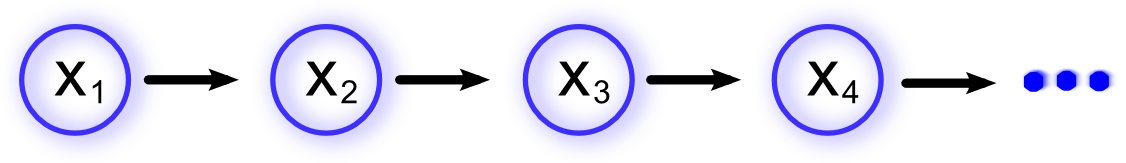
\includegraphics[width=0.4\textwidth]{gfx/mod-mm1}
        \end{center}        
        \begin{equation}
          \label{eqn:2-4}
          p(x_1, ..., x_T) 
            ~=~ \prod_{t=1}^T p(x_T ~|~ x_1, ..., x_{t-1}) 
            ~=~ p(x_1) \cdot \prod_{t=2}^T p(x_T ~|~ x_{t-1}) 
        \end{equation} 
      \item  Se puede generalizar para cadenas de Markov de un orden mayor
        \\~\\
        \begin{center}
          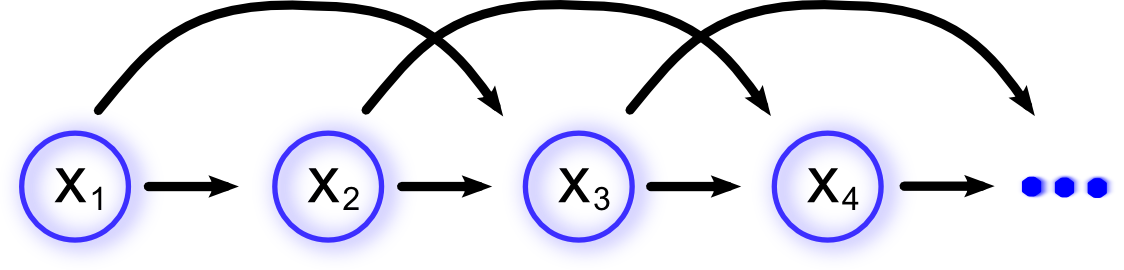
\includegraphics[width=0.45\textwidth]{gfx/mod-mm2}
        \end{center}
        \begin{equation}
          \label{eqn:2-4}
          p(x_1, ..., x_T) 
            ~=~ p(x_1) p(x_2 ~|~ x_1) \cdot \prod_{t=3}^T p(x_T ~|~ x_{t-1}, x_{t-2}) 
        \end{equation} 
  \end{itemize} 
\end{frame}

\begin{frame}{Modelo oculto de Markov}
  \begin{itemize}
    \itemsep1em
    \item Agregar una variable latente $z_t$ (discreta), que corresponda a cada observación $x_t$.
      \begin{align}
        z_{t+1} &\perp z_{t-1} ~|~ z_{t} \\
        p(x_1, ..., x_T, z_1, ..., z_T) &~=~ p(z_1) \left [ \prod_{t=2}^T p(z_t ~|~ z_{t-1}) \right ] 
          \prod_{t=1}^T p(x_t ~|~ z_{t}).
      \end{align}

    \item Modelar proceso bivariado en el tiempo. Una variable observada y una variable latente asociada.
      \\~\\
      \begin{center}
        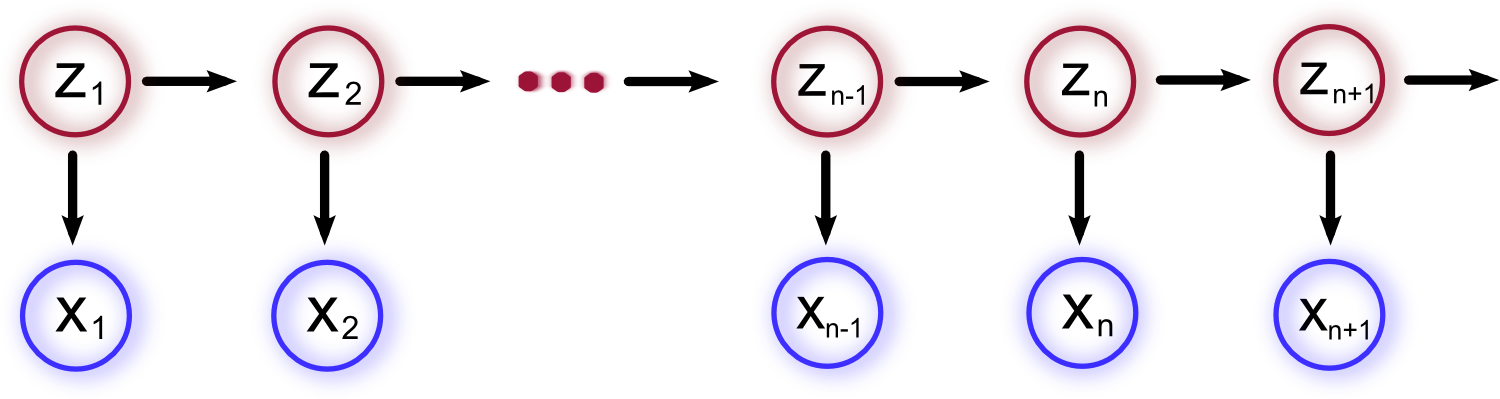
\includegraphics[width=0.5\textwidth]{gfx/mod-hmm}
      \end{center}    
      
    \item Mezcla de distribuciones en la que la densidad está dada por $p(x | z)$      
  \end{itemize}
\end{frame}

\begin{frame}{Parámetros del HMM}
  \begin{itemize}
    \item Probabilidad de cambio entre estados dada una \alert{matriz de transición} $\mathbf{A}$
      \begin{align}
        A_{jk} &\equiv p(z_{tk} = 1 ~|~  z_{t-1, j} = 1) \\
        p(z_t ~|~ z_{t-1}, \mathbf{A}) &= \prod_{k=1}^K \prod_{j=1}^K A_{jk}^{z_{{n-1}, j} \cdot z_{t,k}}
      \end{align}      
    \item \alert{Vector de distribución inicial} $\bm{\pi}$ para variable latente.
      \begin{align}
        \pi_k &\equiv p(z_{1k}) \\
        p(z_1 ~|~ \pi) &= \prod_{k=1}^K \pi_k^{z_{1k}}
      \end{align}       
    \item \alert{Probabilidad de emisión} de una variable observada $x_T$ dada una variable latente $z_T$.
      \begin{equation}
        p(x_t ~|~ z_t, \phi) = \prod_{k=1}^K p(x_T ~|~ \phi_k) ^ {z_{tk}}
      \end{equation}
  \end{itemize}
\end{frame}

\subsection{Resolver HMM con EM}

\begin{frame}{HMM con EM}
  \begin{itemize}
    \item \alert{Probabilidad conjunta del modelo}
      \begin{equation}
        p(\mathbf{X}, \mathbf{Z} ~|~ \theta)        
          = p(z_1 ~|~ \pi) \left[ \prod_{t=2}^T p(z_t ~|~ z_{t-1}, \mathbf{A}) \right]
          \prod_{t=1}^T p(x_t ~|~ z_t, \mathbf{B}, \phi)
      \end{equation}
      
      donde $\mathbf{X} = \lbrace x_1, ..., x_N \rbrace$,~ $\mathbf{Z} = \lbrace z_1, ..., z_N \rbrace$ \\~\\

      y los parámetros del modelo $\theta = \lbrace \bm{\pi}, \mathbf{A}, \mathbf{B}, \phi \rbrace$

    \item Función de verosimilitud completa
        \begin{equation}
          \mathcal{Q}(\theta, \theta^{old}) = \sum_{\mathbf{Z}} p(\mathbf{Z} ~|~ \mathbf{X}, \theta^{old})
              \log p(\mathbf{X}, \mathbf{Z} ~|~ \theta)
        \end{equation}      
  \end{itemize}
\end{frame}    

\begin{frame}{HMM con EM}
  \begin{itemize}      
      \vspace{1.5em}
      \begin{description}
        \item[Probabilidad marginal de una variable latente]
          \begin{equation}
            \gamma(z_t) &= p(z_t ~|~ \mathbf{X}, \theta^{old})
          \end{equation}

        \item[Probabilidad conjunta de dos variables latentes consecutivas]
          \begin{equation}
            \xi(z_{t-1}, z_T) &= p(z_{t-1}, z_T ~|~ \mathbf{X}, \theta^{old})
          \end{equation}
      \end{description}
  \end{itemize}
\end{frame}

\begin{frame}{HMM con EM}
  \begin{itemize}
      \item Prob. marginal de $z_{tk} = 1$, prob. conjunta de $z_{t-1,j}, z_{tk}$
        \begin{align}
          \gamma(z_{tk}) &= \mathbb{E} \left[ z_{tk} \right] = \sum_Z  \gamma(\mathbf{z}) z_{tk} \label{eq-13} \\
          \xi(z_{t-1,j}, z_{tk}) &= \mathbb{E} \left[z_{t-1, j} \cdot z_{tk} \right] = 
            \sum_Z  \gamma(\mathbf{z}) z_{t-1, j} \cdot z_{tk} \label{eq-14}
        \end{align}  
        
        \item Función de verosimilitud completa (reescrita con \eqref{eq-13}, \eqref{eq-14})
          \begin{equation}
            \begin{split}
              \mathcal{Q}(\theta, \theta^{old}) = 
              \sum_{k=1}^K \gamma(z_{1k}) \log \pi_k + 
              \sum_{t=2}^T \sum_{j=1}^K \sum_{k=1}^K \xi(z_{t-1,j}, z_{tk}) \log A_{jk} + \\
              \sum_{t=1}^T \sum_{k=1}^K \gamma(z_{tk}) \log p(x_T ~|~ \phi_k)
            \end{split}
          \end{equation}
          
         \item Parámetros estimados por EM: 
         \begin{equation}
           \pi_k = \frac{\gamma(z_{1k})}{\sum_{j=1}^K \gamma(z_1j)}, ~~
           A_{jk} = \sum_{t=2}^T \frac{\xi(z_{t-1,j}, z_{tk})}{ \sum_{l=1}^K \xi(z_{t-1,j}, z_{tl})}
         \end{equation}
  \end{itemize}
\end{frame}

\begin{frame}{Algoritmo backward-forward}
  \begin{align}
  \gamma(z_t) &= p(z_t ~|~ X) = \frac{p(X ~|~ z_t) p(z_t)}{p(X)} \\
  \gamma(z_t) &= \frac{p(x_1, ..., x_t, z_t)p(x_{t+1}, ..., x_T ~|~ z_t)}{p(X)} \\
  \gamma(z_t) &= \frac{\alpha(z_t) \beta(z_t)}{p(X)} \\  
  \end{align}
  donde 
  \begin{align}
    \alpha(z_t) &\equiv p(x_1, ..., x_t, z_t) \\
    \beta(z_t) &\equiv p(x_{t+1}, ..., x_T ~|~ z_t)  \\
    \alpha(z_t) &= p(x_t ~|~ z_t) \sum_{z_{t-1}} \alpha(z_t ~|~ z_{t-1}) \\
    \alpha(z_1) &= p(z_1) p(x_1 ~|~ z_1) = \prod_{k=1}^K \lbrace {\pi_k p(x_1 ~|~ \phi_k)} \rbrace ^ {z_{1k}}
  \end{align}  
\end{frame}

\begin{frame}{Algoritmo backward-forward}
  \begin{align}
    \beta(z_t) = \sum_{z_{t+1}} \beta(z_{t+1})p(x_{t+1} ~|~ z_{t+1}) p(z_{t+1} ~|~ z_t)
  \end{align}  
\end{frame}